\section{Methodology}
\label{sec:method}

% 3.1 rig, twin and roles; 3.2 model and planner; 3.3 tracker, thrust map, measured pull, model integral, takeoff and
% landing; 3.4 reconfiguration; 3.5 authority and safety; 3.6 method and metrics (17 Oct: the clock-free carry ruler).

This section describes the rig, its twin and who flies what (Section~\ref{sec:overview}); the model and the
planner (Section~\ref{sec:model}); the tracker on each UAV, its thrust map, the measured rod pull, the model
integral, and the procedures that take a flight from the floor into the regime the model covers and back
(Section~\ref{sec:tracker}); the reconfiguration, in both directions (Section~\ref{sec:reconfig}); who owns each
UAV and what keeps the fleet safe when a step fails (Section~\ref{sec:safety}); and the experimental method with
the metrics every result is scored on (Section~\ref{sec:experiments}).

% system_overview.tex -- Methodology 3.1: rig, twin and roles (rewritten 12 Oct 2026 to the thesis plan of
% 11 Oct). The safety paragraph and its label sec:safety moved to authority.tex (3.5); the nodes figure is replaced
% by fig:owners there. The twin's description moved here from simulation.tex with its label sec:simulation. T4 is the
% 17 Oct: plates clockwise from +x, angle = 30 x plate (Wesley 14 Oct; docs/rig/plate_numbering.md); the 7 Oct
% registry rows number plates anticlockwise (old p is (12 - p) mod 12 here).

\subsection{Rig, twin and roles}
\label{sec:overview}

\subsubsection{The rig}
\label{sec:hardware}

All control runs centrally, on one ground computer under ROS~2 (Robot Operating System~2), in a
6\,$\times$\,6\,$\times$\,4\,m motion-capture cage. Motion capture (OptiTrack) is the only sensing: it gives the
pose of each UAV, of the ring and of the newcomer's magnet tip, and nothing on the ring is instrumented; the
velocities and body rates of the UAVs and of the ring are differentiated from the poses. Each UAV's flight
controller runs Betaflight in rate mode, receives a collective throttle and three body-rate stick commands over
its own ExpressLRS (ELRS) radio link at 100\,Hz, and closes only its inner rate loop; the arm switch and the
magnet share the link, and the flight controller's telemetry (battery voltage, flight mode, link quality) comes
back on it. Three nodes do the control (Figure~\ref{fig:owners}, Section~\ref{sec:safety}): a centralised planner
that plans the ring's motion and every rod at 10\,Hz (Section~\ref{sec:controller}), one tracking controller per
UAV at 50\,Hz that turns its share of the plan into radio commands (Section~\ref{sec:tracker}), and a fleet
manager that sequences ARM, TAKEOFF, the trajectory, LAND and the reconfiguration events.

\paragraph{UAVs, rods and ring.} Four UAVs on six-cell batteries, each 0.55\,kg as flown: an airframe and battery of
0.475\,kg plus its rod and magnet. Each carries a rigid rod of 0.55\,m and 0.075\,kg with a ball joint at both
ends; the upper joint sits 4\,cm below the UAV's centre. The ring is 0.86\,kg, 0.51\,m across and 40\,mm thick, with
twelve magnet plates every 30$^\circ$ on its top face at a radius of 0.225\,m. Each rod ends in an electromagnet
that catches on a plate only on contact, holds about 9--10\,N straight off the face and less under a pull across
it, and releases under a jerk rather than under a steady load; [the hold against the angle of pull, to be measured
with a spring scale at 0, 30, 45 and 60$^\circ$ off the plate's axis]. The magnets are held on from
start-up so that a quiet radio link cannot drop the ring, and a magnet is switched off by a channel on its UAV's
own link: that is how a release is commanded, and a release the planner is not told of is made the same way. The
newcomer carries the same rod on a tether that goes slack on the rig once it is free of the ring; in the twin
every link, that tether included, is rigid.

\paragraph{Layouts and plate numbering.} A layout is named by the plates its UAVs stand on, counted clockwise
from plate 0 on the ring's $+x$ axis seen from above, so that plate $k$ sits $30k$ degrees clockwise from $+x$
(Figure~\ref{fig:geometry}); every plate number and angle in this thesis follows that rule. (The collaborator's
code counts anticlockwise: his plate 3 is plate 9 here.) The carriers stand on plates 3, 7 and 11, and the fourth
UAV, the one that leaves and rejoins, on plate 9; its departure leaves an even triangle
(Section~\ref{sec:reconfig}).

% fig_geometry.tex -- M3: payload and rod geometry (TikZ). Dimensions from the rig (30 Sep 2026):
% plates at r 0.225 m on a 500 mm ring, 12 plates every 30 deg, rod 0.55 m, pivot 4 cm below the UAV centre.
% 17 Oct: plates numbered clockwise from +x seen from above (angle = 30 x plate, Wesley 14 Oct); the side view at
% the planned elevation of 60 deg (since 7 Oct). Drawn to scale (1 m = 9 cm).
\begin{figure}[h]
\centering
\begin{tikzpicture}[x=9cm, y=9cm, >=Stealth, font=\small]
  % ---------------- (a) top view ----------------
  \begin{scope}
    \fill[gray!12] (0,0) circle (0.25);
    \fill[white] (0,0) circle (0.19);
    \draw[gray!60, thin] (0,0) circle (0.25) (0,0) circle (0.19);
    % the even triangle left after plate 9 leaves
    \draw[densely dashed, gray!70] (30:0.225) -- (150:0.225) -- (270:0.225) -- cycle;
    % plates, numbered clockwise from +x
    \foreach \k in {0,...,11} {
      \pgfmathsetmacro{\a}{-30*\k}
      \node[draw, fill=white, minimum size=0.11cm, inner sep=0pt, rotate=\a] at (\a:0.225) {};
      \node[font=\scriptsize, text=gray!70!black] at (\a:0.29) {\k};
    }
    % the four carrying plates: 3, 7, 9 and 11
    \foreach \k in {3,7,9,11} { \fill[black] (-30*\k:0.225) circle (0.012); }
    \draw[thick, black] (-270:0.225) circle (0.022);
    % centre, axes, rho
    \fill (0,0) circle (0.008);
    \draw[->, thin, gray] (0,0) -- (0.09,0) node[below, font=\scriptsize, text=black] {$x_L$};
    \draw[->, thin, gray] (0,0) -- (0,0.09) node[left, font=\scriptsize, text=black] {$y_L$};
    \draw[->, thick] (0,0) -- (30:0.213) node[pos=0.62, above left, inner sep=1pt] {$\boldsymbol{\rho}_i$};
    \draw[->, gray] (-12:0.335) arc (-12:-48:0.335);
    \node[font=\scriptsize, text=gray!70!black, anchor=west] at (-30:0.345) {clockwise};
    \node[font=\scriptsize, align=left, anchor=north] at (0,-0.33) {$\bullet$ carrying plates 3, 7, 9, 11\quad $\bigcirc$ plate 9 leaves};
    \node[anchor=north west] at (-0.36,0.36) {(a)};
  \end{scope}
  % ---------------- (b) side view of one rod (A plate, P pivot, C UAV centre), elevation 60 deg ----------------
  \begin{scope}[shift={(0.72,-0.33)}]
    \fill[gray!12] (-0.06,0) rectangle (0.0,0.03);
    \draw[gray!60, thin] (-0.06,0) rectangle (0.0,0.03);
    \fill[black] (-0.012,0.03) rectangle (0.012,0.038);
    \coordinate (A) at (0,0.034);
    \coordinate (P) at (0.275,0.5103);
    \coordinate (C) at (0.275,0.5503);
    \draw[very thick] (A) -- (P);
    \fill (A) circle (0.007) (P) circle (0.007);
    \draw[thick] (0.185,0.5503) -- (0.365,0.5503);
    \draw[gray] (0.185,0.5563) ellipse (0.035 and 0.006) (0.365,0.5563) ellipse (0.035 and 0.006);
    \fill (C) circle (0.006);
    \draw[->, thick] (A) -- (0.08,0.1726) node[pos=0.55, above left, inner sep=1pt] {$\mathbf{q}_i$};
    \draw[gray] (0.16,0.034) arc (0:60:0.16);
    \draw[gray, thin] (A) -- (0.22,0.034);
    \node[font=\scriptsize] at (0.20,0.095) {60$^\circ$};
    \node[font=\scriptsize, anchor=north west] at (0.16,0.30) {$l_i = 0.55$\,m};
    \draw[gray, thin, densely dotted] (P) -- (0.455,0.5103) (C) -- (0.455,0.5503);
    \draw[<->, thin] (0.455,0.5103) -- (0.455,0.5503) node[midway, right, font=\scriptsize] {$\boldsymbol{\delta}$: 4\,cm};
    \node[font=\scriptsize, anchor=north] at (-0.03,-0.005) {ring};
    \node[font=\scriptsize, anchor=south] at (0.275,0.575) {UAV $i$};
    \node[anchor=north west] at (-0.08,0.69) {(b)};
  \end{scope}
\end{tikzpicture}
\caption[Payload and rod geometry]{Payload and rod geometry, to scale. (a) Top view of the 0.86\,kg ring
with its twelve magnet plates at a radius of 0.225\,m, numbered clockwise from the $x_L$ axis seen from above, so
that plate $k$ sits $30k$ degrees clockwise from $x_L$. The four-UAV layout uses plates 3, 7, 9 and 11; when the
UAV on plate 9 leaves, the three on plates 3, 7 and 11 form an even triangle (dashed), under which the ring hangs
level. (b) Side view of one rod at the planned elevation of 60$^\circ$: the rod direction $\mathbf{q}_i$ points
from the plate to the UAV, and the rod pivots $\boldsymbol{\delta}$ = 4\,cm below the UAV's centre.}
\label{fig:geometry}
\end{figure}


\pendingfig{fig:rig_photo}{The rig: four UAVs on rods, the ring with its twelve magnet plates, the motion-capture
markers and the newcomer's magnet tip, with a to-scale top and side view.}{a photograph of the rig, on the next rig day}

\subsubsection{The rig twin}
\label{sec:simulation}

Every controller change is flown in simulation before it reaches the rig, with the same launch files and
controller code. The physics simulator is Gazebo \cite{koenig2004gazebo}, connected to ROS~2
\cite{macenski2022ros2} through bridges. The worlds are generated by a script from the rig's measured geometry
and masses, and each flight starts with the ring on the floor. A flight controller emulator stands in for
Betaflight: it maps the throttle to rotor speed so that thrust follows the rig's identified affine map
(Section~\ref{sec:tracker}), with each UAV's own offset and a battery that sags under load, and closes a
proportional--integral rate loop on the simulated gyro. A motion-capture emulator publishes the simulated poses
on the rig's topics at 120\,Hz. The twin runs at 0.3--0.45 of real time with the full stack on one computer,
under simulated time; wall-clock watchdogs fire when it falls further behind, and such runs are voided and flown
again. The simulator effects that had to be removed before the twin could be trusted are discussed in
Section~\ref{sec:discussion}.

\paragraph{What the twin does not model.} The twin is built from the rig's thrust map, geometry and masses, and
it leaves out six things, each of which the results chapters name where it matters. (i) Loop latency: the rig's
radio and flight controller add about 10--15\,ms to the command path, but the rig turns a throttle command into lift
in 44--67\,ms (nothing on the flight controller closes a loop on collective thrust) against about 15--25\,ms in the
twin, and answers a body-rate command faster than the twin (25--35 against 48--62\,ms); in an exploratory check, 15 and 30\,ms of command delay added in the twin left the carry at 0.3\,m/s
as it was, and 45\,ms tipped a carrier at takeoff. (ii) Solver
timing: in the twin the planner always finishes before its next tick, because simulated time waits for it; on the
rig it has 60\,ms. (iii) Motion-capture noise: the twin's poses are exact. (iv) Rotor wake on the ring and on the
other UAVs. (v) The slack tether: every link is rigid in the twin. (vi) The magnet's holding limit: a twin magnet
never lets go unless commanded. The rig's own measurement had one artefact of its own until the evening of
8 October: body rates were rounded to 0.1\,rad/s on their way to the trackers, and rig flights are labelled before
or after that fix wherever a rate-dependent quantity is compared.

\subsubsection{Roles}
\label{sec:roles}

Two controllers fly in this work, and the division is the same in the twin and on the rig. This work's planner and
trackers carry the ring: the floor start, the carry, the detection of a release, the resize and the redistribution,
the confirmation of an attach from motion capture, the switch of the newcomer's radio, the fold-in, the take-back
and the fault policy. The collaborator's controller flies a free UAV: the pickup of an object with the UAV's
magnet, the transit, the drop into the ring, the descent onto a plate to contact, and the lift that proves the
catch. Where this work's code runs inside the collaborator's stack (the lift from contact, the proof states, the
retry of a pickup, the magnet switched off on a take-back, the check that the object was dropped) it is listed as
this work's, [made with the collaborator's written agreement; the wording of the roles table in the introduction
and of the originality statement is to be agreed with him and the supervisor]. The collaborator's thesis is cited as
in preparation, and his controller is described in this thesis only as far as the admission contract needs
(Section~\ref{sec:reconfig}).


% model.tex -- Methodology: the system model, stated once in the planner's notation.
% Merged 9 Oct (structure audit) from the literature review's payload model (modelling.tex,
% "Cable-Suspended Payload Dynamics") and the planner's model (controller.tex, "Load--cable planner").
% Where the two notations conflicted the planner's is kept. What changed from the review's version:
%  - the rod force T_i is written lambda_i q_i, with q_i pointing from the attachment point to UAV i;
%  - the payload moment is lambda_i rho_i x R_L^T q_i in the payload frame (was rho_i x T_i, frame
%    unstated);
%  - the payload attitude is the quaternion q_L with rotation R_L (was R_L only), and its velocity v_L;
%  - the UAV's equation m_q pddot_i = R_i f_i e3 - m_q g e3 - T_i (scalar thrust f_i along body z) is
%    replaced by the thrust vector f_i each UAV must produce, eq:thrust_req, which is the same equation
%    solved for the thrust; the UAV attitude R_i is then the direction of f_i;
%  - the UAV positions are not states: they follow from the rod kinematics (eq:rod_kin), with the pivot
%    offset delta; the state count is 13 + 14N (the review counted UAV states instead);
%  - a constant force d on the payload is added for steady-error rejection.
% The code (mpc_planner, after Sun et al.) uses s_i = -q_i and t_i = lambda_i.

\subsection{Model and planner}
\label{sec:model}

\subsubsection{System model}

The controller's model follows the load--cable formulation of \cite{tudelft} with the standard
simplifications of Section~\ref{sec:lit_models}: the payload is a rigid body of known mass and inertia,
and each link a rigid, massless rod, taut at all times, whose direction and tension are states. The
formulation calls the links cables, hence the names load--cable planner and cable feedforward (the rod's
planned pull passed to the trackers). The fixed team of the literature
\cite{efficient, wahbaKinodynamicMotionPlanning2024, quan2025swarm} is relaxed so that UAVs can join or
leave mid-flight:
the attachment points and rod lengths are runtime parameters, and the team size selects a solver
(Section~\ref{sec:reconfig}).

The payload has mass $m_L$, inertia $\mathbf{J}_L \in \mathbb{R}^{3\times3}$, position $\mathbf{p}_L$,
velocity $\mathbf{v}_L$, attitude quaternion $\mathbf{q}_L$ (rotation $R_L$) and angular velocity
$\boldsymbol{\omega}_L$ in its own frame. $N$ UAVs pull on it through rods of length $l_i$ attached at
$\boldsymbol{\rho}_i$, offset from the payload's centre of mass (CoM) in the payload frame
(Figures~\ref{fig:geometry} and~\ref{fig:payload_system}). The rod direction $\mathbf{q}_i \in S^2$ points
from the attachment point to UAV $i$, and the rod pulls on the payload with
$\mathbf{T}_i = \lambda_i \mathbf{q}_i$, $\lambda_i \ge 0$.

\begin{figure}[h]
\centering
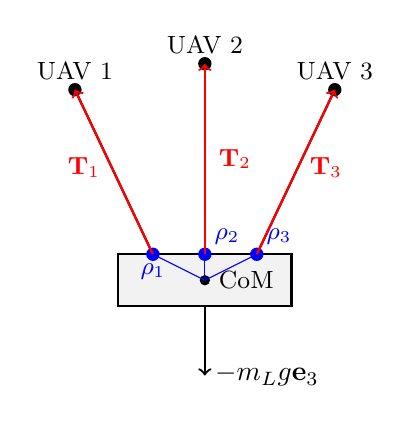
\begin{tikzpicture}[scale=1.1]
  % Payload box
  \draw[thick,fill=gray!10] (-1.0,-0.3) rectangle (1.0,0.3);

  % Centre of mass marker
  \filldraw (0,0) circle (1.5pt);
  \node[right, font=\small] at (0.05,0) {CoM};

  % Gravity
  \draw[->,thick] (0,-0.3) -- (0,-1.1) 
      node[right] {$-m_L g \mathbf{e}_3$};

  % Attachment points on payload surface
  \filldraw[blue] (-0.6,0.3) circle (2pt);
  \filldraw[blue] (0.0,0.3) circle (2pt);
  \filldraw[blue] (0.6,0.3) circle (2pt);

  % UAV 1 - left
  \filldraw (-1.5, 2.2) circle (2pt);
  \node[above, font=\small] at (-1.5,2.2) {UAV 1};
  \draw[thick] (-1.5,2.2) -- (-0.6,0.3);
  \draw[->,red,thick] (-0.6,0.3) -- (-1.5,2.2);
  \node[left, font=\small, red] at (-1.1,1.3) {$\mathbf{T}_1$};
  \draw[->,blue] (0,0) -- (-0.6,0.3) 
      node[below, font=\small, blue] {$\boldsymbol{\rho}_1$};

  % UAV 2 - centre
  \filldraw (0, 2.5) circle (2pt);
  \node[above, font=\small] at (0,2.5) {UAV 2};
  \draw[thick] (0,2.5) -- (0,0.3);
  \draw[->,red,thick] (0,0.3) -- (0,2.5);
  \node[right, font=\small, red] at (0.05,1.4) {$\mathbf{T}_2$};
  \draw[->,blue] (0,0) -- (0,0.3)
      node[above right, font=\small, blue] {$\boldsymbol{\rho}_2$};

  % UAV 3 - right
  \filldraw (1.5, 2.2) circle (2pt);
  \node[above, font=\small] at (1.5,2.2) {UAV 3};
  \draw[thick] (1.5,2.2) -- (0.6,0.3);
  \draw[->,red,thick] (0.6,0.3) -- (1.5,2.2);
  \node[right, font=\small, red] at (1.1,1.3) {$\mathbf{T}_3$};
  \draw[->,blue] (0,0) -- (0.6,0.3)
      node[above right, font=\small, blue] {$\boldsymbol{\rho}_3$};

\end{tikzpicture}
\caption[Multi-UAV payload system]{Multi-UAV payload system: rod $i$ pulls on the payload with tension $\mathbf{T}_i = \lambda_i \mathbf{q}_i$ at the attachment point $\boldsymbol{\rho}_i$, offset from the payload's CoM.}
\label{fig:payload_system}
\end{figure}

Rod $i$ contributes its direction $\mathbf{q}_i$, the angular velocity of that direction $\mathbf{r}_i$
and its first two derivatives, and the tension $\lambda_i$ with its rate:
\begin{equation}
    \mathbf{x} = \big[\, \mathbf{p}_L,\ \mathbf{v}_L,\ \mathbf{q}_L,\ \boldsymbol{\omega}_L,\
    \{\mathbf{q}_i,\ \mathbf{r}_i,\ \dot{\mathbf{r}}_i,\ \ddot{\mathbf{r}}_i,\ \lambda_i,\ \dot{\lambda}_i\}_{i=1}^{N} \,\big]
    \in \mathbb{R}^{13+14N}.
\end{equation}
The inputs are the third derivative of each rod's angular velocity and the second derivative of its
tension, $\mathbf{u} = \{\boldsymbol{\gamma}_i, \eta_i\}_{i=1}^N$, so that the tensions and the rod
directions, and with them the UAV accelerations, are smooth. The dynamics are the payload's
Newton--Euler equations and the rod kinematics:
\begin{align}
    \dot{\mathbf{p}}_L &= \mathbf{v}_L, &
    m_L \dot{\mathbf{v}}_L &= \sum_{i=1}^{N} \lambda_i \mathbf{q}_i - m_L g \mathbf{e}_3 + \mathbf{d},
    \label{eq:plan_trans} \\
    \dot{\mathbf{q}}_L &= \tfrac{1}{2}\, \mathbf{q}_L \otimes \begin{bmatrix} 0 \\ \boldsymbol{\omega}_L \end{bmatrix}, &
    \mathbf{J}_L \dot{\boldsymbol{\omega}}_L &= \sum_{i=1}^{N} \lambda_i\, \boldsymbol{\rho}_i \times R_L^\top \mathbf{q}_i
    - \boldsymbol{\omega}_L \times \mathbf{J}_L \boldsymbol{\omega}_L, \\
    \dot{\mathbf{q}}_i &= \mathbf{r}_i \times \mathbf{q}_i, &
    \dddot{\mathbf{r}}_i &= \boldsymbol{\gamma}_i, \qquad \ddot{\lambda}_i = \eta_i,
\end{align}
where $\mathbf{d}$ is a constant force on the payload, zero in the original formulation and used for
steady-error rejection in Section~\ref{sec:disturbance}. The UAV positions follow from the rod
kinematics,
\begin{equation}
    \mathbf{p}_i = \mathbf{p}_L + R_L \boldsymbol{\rho}_i + l_i \mathbf{q}_i - \boldsymbol{\delta},
    \label{eq:rod_kin}
\end{equation}
with $\boldsymbol{\delta}$ the position of the rod pivot relative to the UAV's
centre ($\boldsymbol{\delta} = -0.04\,\mathbf{e}_3$\,m on the rig). The rod tension couples the system:
it drives the payload in \eqref{eq:plan_trans} and acts, equal and opposite, on UAV $i$.
Differentiating \eqref{eq:rod_kin} twice gives $\ddot{\mathbf{p}}_i$, and the thrust each UAV of mass
$m_q$ must produce is
\begin{equation}
    \mathbf{f}_i = m_q\big(\ddot{\mathbf{p}}_i + g\mathbf{e}_3\big) + \lambda_i \mathbf{q}_i .
    \label{eq:thrust_req}
\end{equation}
The state grows linearly with $N$, which drives the computational scaling noted in \cite{tudelft}.


% controller.tex -- draft of the controller as flown (4 Oct 2026), input from Methodology.tex.
% Notation follows Source/src/model.tex: q_i points from the payload attachment to UAV i and
% T_i = lambda_i q_i. The code (mpc_planner, after Sun et al.) uses s_i = -q_i and t_i = lambda_i.
% Restructured 9 Oct (structure audit): the model moved to model.tex; planner, tracker and steady-error
% rejection are subsections of their own; the result numbers (the box's effect, K's measured values,
% the damping ratio) moved to Section 4.2; the thrust identification procedure moved here from
% hardware.tex; the cost weights moved to Appendix B. Notation: the horizon has N_h nodes over T_h
% (were N and T, which also named the team size and the tension).
% Its references (francis1976internal, pannocchia2003disturbance, pannocchia2007combined,
% maeder2009linear, verschueren2022acados) are in references.bib.

\subsubsection{Load--cable planner}
\label{sec:controller}

The controller is a two-level cascade of model predictive controllers (Figure~\ref{fig:owners}, Section~\ref{sec:safety}).
A centralised planner on the model of Section~\ref{sec:model} plans the motion of the payload and of
every rod over a horizon. Each UAV's tracking MPC follows the planner's reference for that UAV,
accounting for the planned rod force, and sends a collective throttle and three body-rate commands
over the radio link to the flight controller, whose inner rate loop is not modified. Both levels are
solved with acados
\cite{verschueren2022acados} using a real-time iteration (RTI) scheme \cite{diehl2002rti}: one
Gauss--Newton SQP step per tick, warm-started from the previous solution, with the QPs solved by
HPIPM \cite{frison2020hpipm} (partial condensing in the planner, full condensing in the tracker).
Both horizons have $N_h = 20$ nodes over $T_h = 2$\,s. The team size selects the planner's solver and the
attachment geometry is a runtime parameter of it, so that a UAV leaving or joining switches the planner to a
pre-built problem of the new size (Section~\ref{sec:reconfig}); on the rig the planner runs inside the
reconfiguration node, which adds the detection of a release and the resize to the same optimal control problem,
and the rig's carry flights are that node's. On the rig the planner starts no new iteration after 60\,ms of its
100\,ms tick, and a plan that has not converged by then is replaced by the previous one shifted by a tick (the measured
solve times are in Section~\ref{sec:res_compute}).

\paragraph{Optimal control problem.} At each planner tick the planner solves
\begin{equation}
\begin{aligned}
    \min_{\mathbf{x}_{0:N_h},\, \mathbf{u}_{0:N_h-1}} \quad & \sum_{k=0}^{N_h-1} \big\| \mathbf{y}(\mathbf{x}_k, \mathbf{u}_k) - \mathbf{y}_k^{\mathrm{ref}} \big\|_{W}^{2}
    + \big\| \mathbf{y}_{N_h}(\mathbf{x}_{N_h}) - \mathbf{y}_{N_h}^{\mathrm{ref}} \big\|_{W_{N_h}}^{2} \\
    \text{s.t.} \quad & \mathbf{x}_{k+1} = \mathbf{F}(\mathbf{x}_k, \mathbf{u}_k; \mathbf{d}), \\
    & C_0 \mathbf{x}_0 = C_0 \hat{\mathbf{x}}(t), \\
    & \lambda_{\min} \le \lambda_{i,k} \le \lambda_{\max}, \quad f_{\min} \le \|\mathbf{f}_{i,k}\| \le f_{\max}, \\
    & |\boldsymbol{\gamma}_{i,k}| \le \gamma_{\max}, \quad |\eta_{i,k}| \le \eta_{\max},
\end{aligned}
\label{eq:plan_ocp}
\end{equation}
with the output
$\mathbf{y} = [\mathbf{p}_L, \mathbf{v}_L, \mathbf{e}_R, \boldsymbol{\omega}_L, \{\mathbf{q}_i\}, \{\lambda_i\}, \{\mathbf{r}_i\}, \mathbf{u}]$,
where $\mathbf{e}_R = 2\,\mathrm{vec}(\mathbf{q}_L^{\mathrm{ref}} \otimes \mathbf{q}_L^{*})$ is the sign-invariant
attitude error. The thrust bounds are softened with slack. $\mathbf{F}$ is the integrated dynamics
over one node of $T_h/N_h = 0.1$\,s.

The initial-condition constraint pins only what motion capture measures directly: the payload pose
and twist, and each rod direction ($C_0$ selects $\mathbf{p}_L, \mathbf{v}_L, \mathbf{q}_L,
\boldsymbol{\omega}_L, \mathbf{q}_i$). The rod rates, their derivatives and the tensions are free at
node~0, warm-started from the previous solution, because a tension carried over from the last plan
against a measured pose the UAVs did not quite reach makes node~0 inconsistent.

\paragraph{References.} The payload reference $(\mathbf{p}_L^{\mathrm{ref}}, \mathbf{v}_L^{\mathrm{ref}},
\mathbf{a}_L^{\mathrm{ref}})$ comes from the lift schedule and the trajectory, and the rod references
follow from it by flatness. Holding the payload against gravity, its acceleration and the force
$\mathbf{d}$ needs the rods to support the effective gravity
\begin{equation}
    \mathbf{g}_{\mathrm{eff}} = g\mathbf{e}_3 + \mathbf{a}_{L,xy}^{\mathrm{ref}} - \mathbf{d}/m_L ,
\end{equation}
where $\mathbf{a}_{L,xy}^{\mathrm{ref}}$ is the horizontal part of the reference acceleration (the
trajectories are level). The nominal formation (each rod at the planned elevation, 45$^\circ$ until 7 October and 60$^\circ$ since, tensions
$\lambda_i^{0}$ balancing the payload weight) is rotated so that its vertical axis lies along
$\mathbf{g}_{\mathrm{eff}}$, and the tensions are scaled to $\lambda_i^{\mathrm{ref}} = \lambda_i^{0}\,
\|\mathbf{g}_{\mathrm{eff}}\| / g$. Of the weights (Table~\ref{tab:weights}, Appendix~\ref{sec:app_params}),
the one on the rod directions holds the formation's shape and the one on the rod rates damps rod swing.

\paragraph{Output to the trackers.} From the solved horizon the planner sends each tracker, at every node,
its reference position and velocity from \eqref{eq:rod_kin}, the planned thrust per unit mass
$\mathbf{f}_i/m_q$ from \eqref{eq:thrust_req}, whose magnitude is the throttle feedforward and whose direction
the attitude reference, and the planned cable acceleration $\mathbf{a}_{c,i} = -\lambda_i \mathbf{q}_i / m_q$:
twelve numbers per node. The tracker interpolates the whole horizon at its own rate, so a late or skipped
planner tick does not leave it without a reference.

\subsection{Tracker, thrust map, measured pull and model integral}
\label{sec:tracker}

\subsubsection{UAV tracking MPC and thrust map}

Each UAV $i$ runs a tracking MPC on a 17-state model, in which the four stick channels sent to the
flight controller are themselves states and their rates of change are the inputs:
\begin{equation}
    \mathbf{x}_i = [\mathbf{p},\ \mathbf{q},\ \mathbf{v},\ \boldsymbol{\omega},\ \mathbf{c}], \qquad
    \mathbf{c} = [c_\phi, c_\theta, u_T, c_\psi], \qquad \mathbf{u}_i = \dot{\mathbf{c}},
\end{equation}
with
\begin{align}
    \dot{\mathbf{p}} &= \mathbf{v}, &
    \dot{\mathbf{q}} &= \tfrac{1}{2}\, \Omega(\boldsymbol{\omega})\, \mathbf{q}, \\
    \dot{\mathbf{v}} &= R(\mathbf{q})\, k_T u_T \mathbf{e}_3 - g\mathbf{e}_3 - c_z v_z \mathbf{e}_3 + \mathbf{a}_{c,i}, &
    \dot{\boldsymbol{\omega}} &= \frac{1}{\tau_\omega}\big(\boldsymbol{\omega}_{\mathrm{cmd}}(\mathbf{c}) - \boldsymbol{\omega}\big),
    \label{eq:trk_model}
\end{align}
where $\boldsymbol{\omega}_{\mathrm{cmd}}(\mathbf{c})$ is the flight controller's rate curve applied to the
roll, pitch and yaw sticks, and $\tau_\omega$ the time constant of its rate loop. Thrust is affine in
throttle: the throttle sent is $u_T + u_0(V)$, with the offset $u_0(V) = u_0 + \kappa (V_{\mathrm{ref}} - V)$
correcting for the battery voltage $V$ and $k_T$ the gain above it. A proportional map with one gain,
identified at hover, did not hold across loads and battery states, so the map was identified on the
rig: each UAV hovered free with hung masses of 0, 98 and 196\,g over battery voltages of 22.7--24.6\,V,
and its throttle was fitted against the mass it carried and the voltage (Section~\ref{sec:thrust_id}).

The planned cable acceleration $\mathbf{a}_{c,i}$ enters the model as a known, time-varying parameter
along the horizon, so the tracker anticipates the rod's pull instead of reacting to it. The planned pull
is only as good as the planner's model of the rods. On the rig the rods flew at about 60$^\circ$ from
horizontal where the plan assumed 45$^\circ$, so each tracker now measures the pull and uses the plan only
for its shape along the horizon. The measured pull is the UAV's acceleration from motion capture (the
least-squares slope of its velocity over 80\,ms, low-pass filtered at 50\,ms) minus the modelled thrust,
gravity and drag, with the thrust passed through the same filter so that a throttle change does not read
as a change of pull. The horizon's planned pull is shifted by the difference between the measured and the
planned pull at its first node, capped at 12\,m/s$^2$, and the planner plans the rods at 60$^\circ$ to
match (effect on the rig: Section~\ref{sec:res_rig_integral}).

The tracker solves, every 20\,ms,
\begin{equation}
\begin{aligned}
    \min \quad & \sum_{k=0}^{N_h-1} \big\| \mathbf{h}(\mathbf{x}_k, \mathbf{u}_k) - \mathbf{h}_k^{\mathrm{ref}} \big\|_{Q}^{2} + \big\| \mathbf{h}_{N_h}(\mathbf{x}_{N_h}) - \mathbf{h}_{N_h}^{\mathrm{ref}} \big\|_{Q_{N_h}}^{2} \\
    \text{s.t.} \quad & \mathbf{x}_{k+1} = \mathbf{F}_i(\mathbf{x}_k, \mathbf{u}_k; \mathbf{a}_{c,i,k}), \qquad \mathbf{x}_0 = \hat{\mathbf{x}}_i(t), \\
    & 0.05 \le u_{T,k} \le u_{T,\max}, \quad |c_{\phi,k}|, |c_{\theta,k}|, |c_{\psi,k}| \le 1, \quad |\mathbf{u}_k| \le \overline{\mathbf{u}},
\end{aligned}
\label{eq:trk_ocp}
\end{equation}
with $\mathbf{h} = [\mathbf{p}, \mathbf{v}, \boldsymbol{\omega}, \mathbf{c}, \mathbf{u}, \mathbf{e}_R]$, the
attitude reference being the direction of the planned thrust \eqref{eq:thrust_req}. The stick states
are normalised to $[-1, 1]$, and $\overline{\mathbf{u}}$ limits how fast each may change (throttle
0.5\,s$^{-1}$). Only the first command of each solution is sent.

\paragraph{Initial condition.} Node~0 equals the measured state, $\mathbf{x}_0 = \hat{\mathbf{x}}_i(t)$,
the standard formulation, with the stick states taken from the commands actually sent, so the model
starts from where the actuators are. An earlier version relaxed this to the box
$\hat{\mathbf{x}}_i(1-\epsilon) \le \mathbf{x}_0 \le \hat{\mathbf{x}}_i(1+\epsilon)$ with $\epsilon = 0.025$
(Section~\ref{sec:res_ic}).

\subsubsection{The model integral}
\label{sec:disturbance}

Any error that remains constant, from a model mismatch or an external force, is represented by the
constant force $\mathbf{d}$ on the payload in \eqref{eq:plan_trans}. $\mathbf{d}$ is a lumped disturbance:
for an external force (wind, a push, an unmodelled object in the basket) it is that force; for an
internal error (a thrust-map error, the rods' mass) it is the force that would have the same effect on
the payload, which need not exist physically. In the offset-free MPC literature this is an input
disturbance model \cite{pannocchia2003disturbance, maeder2009linear}.

\paragraph{Integral action through the model.} $\mathbf{d}$ is formed from the integral of the payload's
position error $\mathbf{e}_k = \mathbf{p}_L^{\mathrm{ref}} - \mathbf{p}_L$, updated at each planner tick
$k$ (period $T_s = 0.1$\,s):
\begin{equation}
    \mathbf{b}_{k+1} = \mathrm{sat}_{\bar{b}}\!\big(\mathbf{b}_k + k_i T_s\, G_k\, \mathbf{e}_k\big), \qquad
    \mathbf{d}_k = -K \mathbf{b}_k, \qquad K = \mathrm{diag}(K_{xy}, K_{xy}, K_z).
    \label{eq:lumped_int}
\end{equation}
Here $\mathrm{sat}_{\bar{b}}$ bounds each component to $\pm\bar{b}$, and the gate $G_k = \mathrm{diag}(g_{xy},
g_{xy}, g_z) \in \{0,1\}^3$ integrates only in steady, taut flight: lift complete, not descending or
landing, every rod taut, a fresh pose, the payload slow ($<0.05$\,m/s) and the miss under 0.25\,m. The
vertical component also integrates through a slow level orbit; the horizontal components require a
stationary reference, so a value learned in hover is held through a trajectory. A low payload ($e_z > 0$)
makes $d_z$ negative: the planner then believes the payload is heavier and plans more rod tension. Once
the payload rests on the floor at landing, $\mathbf{d}$ is set to zero. $K$ converts the integral from
metres to newtons and is set to the closed-loop stiffness of the cascade to a force on the payload,
measured from the steady displacement under a known force with the planned rod pull (Appendix~\ref{sec:app_params});
the integral's loop gain is then $k_i$, as in the reference-shift form below.

$\mathbf{d}_k$ is a parameter of the planner's problem, constant over the horizon and refreshed at every
tick. It enters the payload's translational dynamics \eqref{eq:plan_trans}, so the plan predicts the
payload's motion with the force included and chooses tensions and UAV positions that counter it. It also
enters the reference formation through $\mathbf{g}_{\mathrm{eff}}$, so the formation the cost draws the
solution towards is already tilted and tensioned to balance $\mathbf{d}$ and the cost does not oppose the
force balance.

\paragraph{Properties.} At an equilibrium with the gate open ($G = I$) and no component of $\mathbf{b}$
saturated, $\mathbf{b}_{k+1} = \mathbf{b}_k$ gives $\mathbf{e} = \mathbf{0}$, whatever the constant cause:
by the internal model principle \cite{francis1976internal}, the integrator is the model of a constant.
This assumes stability; it does not give it. Approximating the cascade's response to $\mathbf{d}$ by a
first-order lag with time constant $\tau$, each axis becomes
\begin{equation}
    \tau s^2 + s + k_i = 0, \qquad \zeta = \frac{1}{2\sqrt{k_i \tau}},
\end{equation}
so a faster integral costs damping, and delays through the planner and the radio link reduce the margin
further. Let an unmodelled constant force
$\mathbf{F}$ act on the payload and let the cascade, of actual stiffness $K_c$, be quasi-static (fast
compared with the integral). The plan cancels the force it believes in, so the payload settles at
$\mathbf{e} = -K_c^{-1}(\mathbf{F} - \mathbf{d}) = -K_c^{-1}(\mathbf{F} + K\mathbf{b})$, and in continuous time
\begin{equation}
    \dot{\mathbf{b}} = k_i\,\mathbf{e} = -k_i K_c^{-1}\big(K\mathbf{b} + \mathbf{F}\big)
    \quad\Rightarrow\quad \mathbf{b} \to -K^{-1}\mathbf{F}, \qquad \mathbf{d} \to \mathbf{F},
\end{equation}
a first-order convergence at the rate $k_i K K_c^{-1}$ on each axis, with time constant $1/k_i = 2.5$\,s when
$K = K_c$. The believed force converges to the applied one whatever $K$ is: $K$ sets only the speed, and
too large a $K$ costs damping as too large a $k_i$ does. When the force is removed, $\mathbf{b}$ still holds
$-K^{-1}\mathbf{F}$, so the payload overshoots by $K_c^{-1}\mathbf{F}$, the displacement the force caused at
onset, and the overshoot decays at the same rate. This analysis assumes that the force reaches the payload's
position error. With the measured rod pull (Section~\ref{sec:tracker}) a constant vertical force is taken up at
each UAV within about a second, before the integral can act, so in the twin the integral is left with the
horizontal axes (Section~\ref{sec:res_force}).

\paragraph{Reference-shift form.} An earlier version added the height integral to the payload's height
target instead, $z_L^{\mathrm{ref}} \leftarrow z_L^{\mathrm{ref}} + b_z$. Both forms reach the same steady
state; in offset-free MPC they are output and input disturbance models, which differ in the transient, not
in the steady state \cite{pannocchia2007combined}. The model form keeps the target fixed, so its plan
predicts a payload held at the target, which is what happens; the reference-shift form plans a move towards
a shifted target that never comes. The model form also extends to the horizontal axes, and it is the
default everywhere, a resizing fleet included (the integral's force is kept through the resize). The
reference-shift form, on the height only, flies where the model form cannot, and flew on the rig on 1 and
8 October ($k_i = 0.4$\,s$^{-1}$); the 7 October carry flights flew the model form.
% Model integral through a resize since 8 Oct (896aff2; bringup real_mode.planner_options).
% STATUS 5 Oct 2026: int_mode auto (model where allowed, else reference): reference with kt_trim on,
% a resizing fleet, z_ki 0, offset_free on or dist_est ring/full (bringup real_mode.planner_options).

\paragraph{Bound and limits.} $\bar{b} = 0.3$\,m bounds the force the integral can supply to $K\bar{b}$
(2.1\,N vertically), enough for an unmodelled 0.1\,kg object. A larger error is a fault, not a disturbance,
and a warning at 70\,\% of the bound reports it rather than covering it silently; the bound and the warning are
also what stop an integral that winds up without effect, as the vertical integral does on a wrong attachment
radius in the twin (Section~\ref{sec:sim_robustness}). A force on the payload cannot represent a moment: one UAV's
thrust-map error is a moment on the ring, which that UAV's own tracker takes up through its measured pull. A miss
larger than the gate is never integrated. The integral is also slow ($1/k_i = 2.5$\,s): it removes constant and
slowly varying forces, not impacts or gusts. Five other ways to remove a steady error were built and flown on the
earlier stack (a force balance \cite{muske2002disturbance}, an offset-free observer
\cite{pannocchia2003disturbance}, the measured cable force, a per-UAV thrust-gain trim, and the rods' mass in the
planner); Appendix~\ref{sec:app_methods} records them, and the measured cable force became the trackers' measured
pull.


% takeoff_landing.tex -- Methodology: takeoff from the floor, lift and landing (draft 4 Oct 2026).
% Code: mpc_planner/creep_controller.py (arc creep, hand-over latch), planner_node.py (pretension,
% breakaway, ff_cap_release_s, lift ramp, LAND, TouchdownDetector), bringup/config/*.yaml.
% Evidence: 23 Sep rig non-lift (start_taut), 30 Sep rig review, R0817/R0818, R0834-R0839 (B2),
% R0807-R0816 (hand-over angle in the twin), RIG-1001-* (hand-over and rods on the rig).
% Condensed 12 Oct 2026 to the plan's half page; the detail is Appendix C "Floor start and landing in detail".
% Restructured 9 Oct (structure audit): the outcomes (the hand-over angle flown, fig:flight) moved to
% Section 4.1.

\subsubsection{Takeoff, lift and landing}
\label{sec:takeoff}

The planner assumes taut rods, but every flight starts and ends with the ring on the floor and the rods slack or
flat, where the UAVs sit about 0.7\,m from the ring's centre, outside the cone the planner's references put them
on; started from rest, the planner pulled the UAVs inwards over the ring instead of lifting it, the cause of the
first failed lifts on the rig. Four steps take a flight from the floor into the regime the planner models, and three
measures take it back; Appendix~\ref{sec:app_floor} gives each with its numbers and the failure it answers.
\begin{itemize}
    \item \textbf{Rod sweep.} On TAKEOFF each UAV is anchored where it rests and its rod is swept about its own
    attachment point from its measured elevation to the planned one (60$^\circ$ since 7 October), the UAV's
    reference riding the far end of the rod, so that the rod stays straight and the UAV never crosses over the
    ring. The planner takes over once every rod has held within 8$^\circ$ of the planned elevation for 1\,s, and
    measures each rod's length from motion capture at that hand-over for its model and its tautness gate.
    \item \textbf{Pretension and breakaway.} Every UAV's share of the planned pull then rises together from zero
    over 3\,s with the ring's height target at its resting height; a step here launched the ring and released two
    magnets on the rig. When the ring rises 1\,cm or faster than 0.03\,m/s it has broken free, and the fraction of
    the planned pull reached at that moment is frozen as a cap on the trackers' feedforward, released back to the
    full pull over 2\,s once the lift starts.
    \item \textbf{Lift.} The height target ramps to the target height at 0.1\,m/s, eased in and out, and the
    trajectory starts when the ramp completes.
    \item \textbf{Landing.} On LAND the ring's height target descends at 0.2\,m/s with the formation unchanged
    until the ring rests. A rigid rod then pushes a UAV descending straight down outward as the rod lengthens
    horizontally, which tipped UAVs over in the twin, so each UAV's reference unwinds along its rod's circle about
    the grounded attachment point before it descends (twin only: the rig's tethers go slack and it lands straight
    down); the planner blends each UAV's thrust and rod feedforward to plain hover over 1\,s instead of dropping
    the rod term at touchdown; and a UAV back at its resting height with the ring down idles armed until the fleet
    disarms, so that a UAV that lands first does not track a reference below the floor. Touchdown is declared when
    the UAVs stop following the descending reference for 1\,s after at least 5\,cm of descent, and the fleet
    manager disarms the fleet. In the twin this stall test is re-armed when the ring touches down, so that the
    second in which the UAVs blend from carrying to free hover cannot read as a stall: without the re-arm a
    landing could disarm the fleet with the UAVs 0.4--0.5\,m up (Section~\ref{sec:sim_landing}). On the rig the
    re-arm waits for a review of its pose-freshness check.
\end{itemize}


% reconfiguration.tex -- Methodology 3.4: reconfiguration (rewritten 12 Oct 2026 to the thesis plan of 11 Oct:
% notice, re-plan, redistribute, fall back; the three-equation statics; the support margin with its qualifier; the
% constants table; the admission contract; the state machine). 17 Oct (v3): the join is noticed by the co-motion
% confirmation (the default since 14 Oct, proof_rules comotion; card docs/experiments/2026-10-15_attach_comotion_rig.md
% rev 4, Tejen's review); the old contact-and-lift proof is history. Plates clockwise (angle = 30 x plate).
% Code: the planner's detach mode (detection, resize), drone_magnet (contact proof, attachment manager, radio mux),
% the take-back in the tracker; the collaborator's stack carries the lift from contact.

\subsection{Reconfiguration}
\label{sec:reconfig}

A reconfiguration changes the number of UAVs carrying the ring in the air. Both directions are handled by the same
four steps: the planner \emph{notices} the change from an observation, \emph{re-plans} by switching to a solver
built for the new team, \emph{redistributes} the ring's weight across it, and \emph{falls back} to a simple exit
when a step fails. Figure~\ref{fig:reconfig_states} shows the two lanes and their exits; the constants every step
uses are in Table~\ref{tab:constants}, each with the reason for its value.

\begin{figure}[htbp]
\centering
\begin{tikzpicture}[>=Stealth, font=\small,
    st/.style={draw, thick, rounded corners=3pt, align=center, minimum height=0.8cm, minimum width=2.2cm, font=\small},
    ours/.style={st, fill=blue!6, draw=blue!50!black},
    his/.style={st, fill=orange!10, draw=orange!60!black},
    exit/.style={st, fill=gray!14, draw=gray!60},
    ev/.style={font=\scriptsize, align=center}]
  % leave lane (top)
  \node[ours] (carry)   at (0,0)      {Carry, $N$ UAVs\\ \scriptsize planner owns the ring};
  \node[ours] (resize)  at (4.8,0)    {Resize to $N-1$\\ \scriptsize warm start, free tensions};
  \node[ours] (carry3)  at (9.6,0)   {Carry, $N-1$\\ \scriptsize statics sets the shares};
  \node[ours] (freed)   at (4.8,-1.7) {Freed UAV\\ \scriptsize steps out 0.5\,m};
  \node[exit] (dland)   at (9.6,-1.7){Lands by itself\\ \scriptsize disarmed alone at rest};
  \draw[->, thick] (carry) -- node[ev, above] {DETACH, or\\ rod stretch} (resize);
  \draw[->, thick] (resize) -- (carry3);
  \draw[->, thick] (resize) -- node[ev, right] {the leaver} (freed);
  \draw[->, thick] (freed) -- (dland);
  % join lane (middle)
  \node[his]  (mission) at (0,-3.6)   {Newcomer, free\\ \scriptsize collaborator's controller};
  \node[his]  (contact) at (4.8,-3.6) {Descent to contact\\ \scriptsize then a small lift};
  \node[ours] (proof)   at (9.6,-3.6){Confirmed by mocap\\ \scriptsize tip moves with the plate};
  \node[ours] (takeback) at (4.8,-5.3){Take-back\\ \scriptsize moved clear, lands alone};
  \node[ours] (fold)    at (9.6,-5.3){Mux switch, fold in\\ \scriptsize seed 0.1\,N, resize to $N+1$};
  \draw[->, thick] (mission) -- node[ev, above] {transit\\ to the plate} (contact);
  \draw[->, thick] (contact) -- node[ev, above] {contact} (proof);
  \draw[->, thick] (proof) -- node[ev, right] {confirmed} (fold);
  \draw[->, thick, dashed] (contact) -- node[ev, right] {give-up} (takeback);
  \draw[->, thick, dashed] (proof.south west) -- node[ev, sloped, above, pos=0.45] {not confirmed} (takeback.north east);
  \draw[->, thick] (fold.east) -- ++(0.55,0) |- node[ev, pos=0.25, right] {carry, $N+1$} (carry3.east);
  % exits (bottom)
  \node[exit] (drop) at (0,-7.0)    {Drop and land\\ \scriptsize second loss, or tilt $>$ 30$^\circ$};
  \node[exit] (cut)  at (4.8,-7.0)  {Tilt cut\\ \scriptsize newcomer's motors off};
  \node[exit] (land) at (9.6,-7.0) {LAND\\ \scriptsize every UAV, from any phase};
  \draw[->, thick, dashed] (takeback) -- node[ev, right] {stuck, tilting} (cut);
\end{tikzpicture}
\caption[Leave and join lanes and their exits]{The leave lane (top), the join lane (middle) and the exits
(bottom). Blue: this work's planner and trackers; orange: the collaborator's controller; grey: an exit that ends
with every UAV owned and on the floor. A leave is noticed from the DETACH command or from the leaver's rod reading
longer than itself; a join from a contact and, after the collaborator's lift, the magnet tip seen moving with the
plate on a taut tether, from motion capture alone. Every exit is reachable from every state: LAND and the drop rule
are not drawn into each.}
\label{fig:reconfig_states}
\end{figure}

\subsubsection{Notice}

\paragraph{A leave.} An \emph{announced} leave is the DETACH command: the leaver's magnet is switched off on its
radio channel and the planner resizes on the same tick, or, for a \emph{ramped} release, its planned tension is run
down over a short ramp before the magnet is released, so that the survivors take up the share before the rod goes.
An \emph{unannounced} leave is a magnet switched off without the planner being told, which is how a release the
planner does not expect is made on the rig and in the twin. The planner notices it from the rod: a rigid rod on its
plate cannot measure longer than itself, so when the leaver's rod, measured from motion capture between its pivot
and its plate point, reads more than 0.06\,m over its length for two consecutive ticks, the planner drops that UAV
from its problem. Nothing else is needed: no force sensor, no message from the leaver.

\paragraph{A join.} A join is noticed in two steps, both read from motion capture and nothing else, with the
magnet tip expressed in the plate's own frame. A \emph{contact} is the tip inside the catch radius of the plate
point (24\,mm on the rig), between 15\,mm below and 12\,mm above the plate's face, and slower than 0.03\,m/s for
0.3\,s. A contact is only a candidate: a tip resting on the plate and a magnet that has caught look alike. The
\emph{confirmation} uses the collaborator's small lift: 1.0\,s after its controller signals the lift done, the catch
is confirmed if the tip has stayed within 6\,mm of its contact point while the plate has moved with it (a range of
5\,mm or a rise of 3\,mm), the tip is within 10\,mm of the plate's face, and the tether reads taut against the free hang measured on the
same flight (within 3\,mm). A separation of 45\,mm for 0.12\,s fails it, and no hold spans missing data: a gap of more than 0.1\,s
restarts the contact and the confirmation. In the twin, whose stiff ring hardly moves and whose magnet catches at the
instant of contact, the plate-motion condition is waived and the face window is 15\,mm instead of 10. Until 14 October the proof
asked instead for the tip-to-plate vector to stay within 3\,mm while the plate rose 3\,mm; on the rig it rejected the
one catch of 14 October on its taut check, and this co-motion confirmation replaced it.

\subsubsection{Re-plan}

The planner keeps flying the ring and re-solves for the new team, which two properties of the formulation make
possible. The attachment points $\boldsymbol{\rho}_i$ and rod lengths $l_i$ are runtime parameters of the model, not
constants compiled into the solver, so only the team size fixes the problem's dimensions, and one solver per team
size, built in advance and primed twice on the measured state before it flies, covers any layout. And the
survivors keep their own attachment points, plates 3, 7 and 11 when the carry layout loses plate 9: the planner's
nominal tensions come from a moment balance at the actual plates, so the ring's reference stays level, whereas a
re-spaced even ring would make the moment balance wrong by construction. At the event the planner swaps to the
solver for the new size, sets the attachment points and rod lengths (for a newcomer, the plate it caught, recorded
in the ring frame at the confirmation), and warm-starts the new problem from the measured state with the tensions
and rod directions free at its first node (Section~\ref{sec:controller}); the first solve redistributes the load,
and there is no separate hand-off phase. An announced leave is refused during LAND and when it would leave fewer
than three UAVs, since a rigid ring on two rim points is a pendulum about the line between them; an unannounced
loss that leaves fewer than three is a fault, which drops the ring (Section~\ref{sec:safety}).

\subsubsection{Redistribute}

\paragraph{What statics fixes.} With three carriers the vertical shares are not the planner's to choose. Take the
ring's centre of mass as the origin of its frame and the survivors' plates at $\boldsymbol{\rho}_i = r(\cos\alpha_i,
\sin\alpha_i, 0)$; with $f_i$ the vertical component of rod $i$'s pull on a level ring, the force balance and the
two moment balances about the horizontal axes are three equations in three unknowns,
\begin{equation}
    \sum_{i=1}^{3} f_i = m_L g, \qquad \sum_{i=1}^{3} f_i \cos\alpha_i = 0, \qquad \sum_{i=1}^{3} f_i \sin\alpha_i = 0,
    \label{eq:statics}
\end{equation}
whose solution is unique whenever the three plates do not lie on a line: each share is the weight times the
barycentric coordinate of the centre of mass in the survivors' triangle. The rods' horizontal components, which the
planner does set through the rod directions, balance one another and make no moment about the centre of mass when
the centre lies in the plates' plane \cite{michael2011cooperative, tognon2018internal}; on the
ring the plates sit 2\,cm above the centre of mass, so the shares of \eqref{eq:statics} hold to within a few per
cent. After a leave the planner's first solve therefore hands the leaver's share to the survivors as
\eqref{eq:statics} says (Figure~\ref{fig:detach}). A level ring is possible only when every $f_i$ is positive, which
is the condition of the next paragraph.

\paragraph{Support margin.} A rigid payload can hang level from three or more rim points only if its centre of mass
lies inside the polygon of the attachment points \cite{michael2011cooperative}. For plates on a ring of radius $r$
the nearest edge of the survivors' polygon is the chord across their largest angular gap $g_{\max}$, and the
distance from the centre to that chord,
\begin{equation}
    m = r \cos\!\big(g_{\max}/2\big),
    \label{eq:margin}
\end{equation}
is the support margin: positive inside, zero on the edge, negative outside. On the 0.225\,m plate radius a gap of
120, 135, 150, 165 or 180$^\circ$ leaves a margin of 112, 86, 58, 29 or 0\,mm. Removing one carrier from an even
ring of $N$ leaves a largest gap of $4\pi/N$, which keeps the centre inside only for $N \ge 5$; an even ring of
four sits exactly on the boundary after any loss, which is why the four-UAV flights use plates 3, 7, 9 and 11,
where the loss of the carrier on plate 9 leaves an even triangle with a 112\,mm margin. The margin is the lever the
results chapter varies in the twin (Section~\ref{sec:res_leave}).

\paragraph{Which carrier may leave, and what control still sets.} The condition also says which carriers a layout
can afford to lose, and it can be checked before a flight from the plate angles alone. Removing one carrier merges
the two angular gaps on either side of it, and the four gaps of a four-carrier layout sum to $360^\circ$, so some
pair of adjacent gaps sums to at least $180^\circ$: no four-carrier layout on the ring can lose an arbitrary
carrier and still hang level, and a layout admits at most two leavers. The carry layout admits exactly one, the
carrier on plate 9; losing the carrier on plate 7 or plate 11 puts the centre on an edge, and losing the one on plate
3 puts it 112\,mm outside. The layout on plates 3, 6, 9 and 11 admits the same leaver with a $150^\circ$ gap and a
58\,mm margin. A team that must tolerate the loss of any one carrier therefore needs five, and a four-carrier layout
is designed for a known leaver, which is what the rejoin mission does.
% The numbers: tools/admissibility_map.py (results/analysis/admissibility/), from metrics.cog_margin and the
% planner's balanced_tensions; 0 of the 495 four-plate layouts admits every leaver (11 Oct).
Once the leaver has gone, what control can still set is bounded by the same statics. With three survivors no
controller can change how the ring's weight is shared. What the planner does set is the margin, through the choice
of layout and leaver before the flight; when and how fast the survivors take up the step, since an announced leave
can be ramped while an unannounced one is taken up at the detection; the rods' directions, which fix the horizontal
balance and where the survivors fly; and the ring's position and height through the transient. With four or more
carriers the tensions have a one-parameter family of solutions and the planner takes the split closest to equal
shares, so there a level ring can be held with more than one distribution.

\paragraph{The ramp and the seed.} Where the planner is told of a change it can shape the step. For a ramped
release the leaver's planned tension is run down and the survivors' run up over a short ramp before the magnet is
released, in place of a step at the resize tick; the first version of the ramp, which ran the leaver's tension
down but let the survivors' step, is the negative that defined it. For a join the newcomer is seeded at 0.1\,N and
every tension is blended to the balanced solution for the new geometry, as a dock blends thrust across its
controller switch \cite{sugihara2023trady}: on the earlier plant a newcomer started at a full share pulled the ring
with a lever about the incumbents' rod apex and tilted it at the weld (Appendix~\ref{sec:app_proximity_weld}).

\subsubsection{Fall back}

\paragraph{The freed UAV.} After a release the freed UAV steps 0.5\,m out radially at its height, clear of the ring
and the survivors, and lands by itself while the survivors carry on: its height reference is pressed below its own
resting height until it is there, and it is then disarmed alone, without waiting for the fleet
(Section~\ref{sec:res_freed}). Touchdown for the fleet is judged on the survivors only, so a freed UAV still
descending elsewhere does not hold their references down, and the fleet is declared landed only when it is down
too; the rod feedforward is switched off once the ring rests, because its sideways component pushes a grounded
survivor across the floor.

\paragraph{The take-back.} A newcomer whose contact is not confirmed within its timeout, or whose controller gives
up, is taken back: this work's tracker latches onto its measured position and velocity, ramps its reference at
0.25\,m/s$^2$ so that the latch makes no step, lifts it clear of the rim and the carriers, moves it out and lands it
by itself. On the circle the hold moves with the ring in the ring's planned frame, so that an orbiting formation
cannot sweep a carrier into the newcomer's rod; where the newcomer is low and far out, it lands where it stops. On
the rig the take-back first rises only 5\,cm above the tether's slack and waits for the tip to leave the plate, so
that a magnet that has caught after all is not torn off; if the plate rises instead, the magnet is switched off
again and the fleet lands. The tilt cut, the drop rule and LAND are the exits of Section~\ref{sec:safety}.

\subsubsection{The admission contract}
\label{sec:admission}

The join is a contract between two controllers, and this work's side of it is written so that nothing on the
newcomer's side has to be trusted. The collaborator's controller, which flies the newcomer to the ring, must:
descend onto its plate to contact with the magnet on (on the rig it waits at the bottom with the magnet on until a
contact is seen); lift by a small set amount and hold; signal that the lift is done; and give up its authority when
the catch is confirmed, or give up and go home. This work must: observe the contact and the lift from motion capture
only (the tip in the plate's frame, its drift from the contact point, the plate moving with it and the taut
tether); switch the newcomer's radio to its own tracker on the same tick as the confirmation; fold the newcomer in
from 0.1\,N; and take it back if nothing is confirmed. The multiplexer in front of the newcomer's radio forwards the
collaborator's commands until the confirmation, switches only onto a command that is armed and above idle throttle
(a switch onto an idle stream cut the newcomer's motors at every weld in early tests), and latches; an abort latches
it to a disarmed idle command until it is restarted. The fold-in records the plate in the ring frame, switches the
planner to the solver for $N+1$, and the trajectory continues. Section~\ref{sec:res_join} scores the contract on what
each side costs the ring: the time from contact to confirmation, the ring's tilt rise and dip through the admission,
the step in the newcomer's commands at the switch, and the clearances.

\paragraph{The rejoin mission.} The full mission is assembled with the collaborator's mission planner. Four UAVs
carry the ring in hover or round the circle; the one on plate 9 is released and flies the collaborator's errand
(picking up an object with its magnet and dropping it into the ring) and comes back to its plate; it is admitted
under the contract above, folded in, and the fleet lands. On the rig the collaborator's controller does every
attach down to contact, since the magnet catches only on the plate; this work's own approach, which steered the
measured magnet tip and welded on proximity, flies in the twin only (Appendix~\ref{sec:app_proximity_weld}).

\begin{table}[htbp]
\centering
\small
\caption[Reconfiguration constants and their reasons]{The constants of the reconfiguration and the reason for each
value: a noise floor times a factor, or a physical bound. [Bracketed reasons wait for the offline sweeps over the rig
recordings.]}
\label{tab:constants}
\begin{tabularx}{\textwidth}{>{\raggedright\arraybackslash}p{3.6cm}>{\raggedright\arraybackslash}p{2.4cm}>{\raggedright\arraybackslash}X}
\toprule
Constant & Value & Reason \\
\midrule
Rod stretch for an unannounced leave & 0.06\,m, two ticks & A rod on its plate cannot read longer than itself; the
threshold sits above the scatter of a rod length measured from motion capture, and two ticks reject a single bad
pose. [False alarms over the rig recordings and delay against threshold from the rig releases.] \\
Contact & catch radius 24\,mm (rig); face $-15$ to $+12$\,mm; under 0.03\,m/s for 0.3\,s & The magnet catches only on
the plate: the tip must be over the plate's face and at it, and still for 36 motion-capture samples, which excludes a
pass over the plate. \\
Confirmation, 1.0\,s after the lift & tip within 6\,mm of its contact point; plate range 5\,mm or rise 3\,mm; taut
within 3\,mm & A caught tip moves with the plate and a missed one is left behind by it; the free hang is measured on
each flight, so the taut check reads this flight's tether. \\
Confirmation fails & 45\,mm for 0.12\,s; any data gap over 0.1\,s restarts & A tip that leaves the plate has not
caught; no hold is judged across missing poses. \\
Newcomer's seed tension & 0.1\,N & Small against the newcomer's balanced share (1.6\,N on plate 9 of the carry
layout), so the fold-in's blend and not the weld sets the step. \\
Step-out after a release & 0.5\,m radially & Clears the rim (0.255\,m) and the survivors' rods from the leaver's
plate. \\
Take-back ramp & 0.25\,m/s$^2$ & A quasi-static tilt of 1.5$^\circ$ on the newcomer, under the 2$^\circ$ bar on its
attitude step, and it stops 0.34\,m/s in 1.4\,s. \\
Take-back clearances & 0.15\,m over the carriers; 0.3\,m under the ring; 0.9\,m from the ring's centre & The
newcomer's body and rod stay a rotor disc clear of the carriers; a low newcomer lands where it is rather than
rising through the formation. \\
Ring tilt that drops the ring & 30$^\circ$ & Beyond the planner's near-level model and about where a rod's pull turns
across its plate; where the controller gives up, not a value to design to (Section~\ref{sec:safety}). \\
Fewest carriers & 3 & Two rim points make the ring a pendulum about the line between them. \\
\bottomrule
\end{tabularx}
\end{table}


% authority.tex -- Methodology 3.5: authority and safety as runtime assurance (drafted 12 Oct 2026 from the thesis
% plan of 11 Oct). The safety paragraph moved here from system_overview.tex (its label sec:safety comes with it);
% fig:owners (F5) replaces the old nodes and cascade figures. The rig switch states in brackets follow plan D6 and
% the M1 plan's D6(a)/(b): they are set per lab day and are not results.

\subsection{Authority and safety}
\label{sec:safety}

Every UAV in the air has exactly one controller sending it commands at every instant, and every phase has a way
down that ends with the UAV disarmed on the floor. Figure~\ref{fig:owners} shows the cascade and who owns what.
The planner owns the ring: it plans the ring's motion and every rod, and hands each carrier's share to that
carrier's tracker. A tracker owns its UAV's radio link; nothing else writes to it. A UAV that is not on the ring
is owned either by its own tracker (a freed carrier landing by itself, a newcomer being taken back) or by the
collaborator's controller (the newcomer through its pickup, transit, drop and descent to contact), and the
multiplexer in front of the newcomer's radio is the one place where ownership changes hands: it forwards the
collaborator's commands until the attach is confirmed, switches to this work's tracker on that tick, and latches.
Below the trackers each flight controller closes only its body-rate loop and arms, disarms and switches its magnet
on channels the tracker sets; the operator holds a disarm button that overrides everything.

\begin{figure}[htbp]
\centering
\begin{tikzpicture}[>=Stealth, font=\small,
    blk/.style={draw, thick, rounded corners=2pt, align=center, minimum height=0.85cm, font=\small},
    ours/.style={blk, fill=blue!6, draw=blue!50!black},
    his/.style={blk, fill=orange!10, draw=orange!60!black},
    fc/.style={blk, fill=gray!12, draw=gray!60},
    lab/.style={font=\scriptsize, align=center}]
  \node[blk]  (op)   at (5.6,1.7)   {Operator\\ \scriptsize disarm button};
  \node[ours] (fm)   at (5.6,0)     {Fleet manager\\ \scriptsize phases, faults, LAND};
  \node[ours] (plan) at (0,0)       {Load--rod planner\\ \scriptsize 10\,Hz; owns the ring};
  \node[ours] (trk)  at (0,-2.5)    {Tracker $i$ (carrier)\\ \scriptsize 50\,Hz; owns UAV $i$};
  \node[ours] (trkn) at (5.6,-2.5)  {Tracker (newcomer)\\ \scriptsize from the attach, or take-back};
  \node[his]  (tej)  at (11.3,-2.5) {Collaborator's controller\\ \scriptsize pickup, transit, drop,\\ \scriptsize descent to contact, lift};
  \node[ours] (mux)  at (5.6,-4.6)  {Mux\\ \scriptsize one owner, latched};
  \node[fc]   (bf)   at (0,-4.6)    {Flight controller $i$\\ \scriptsize Betaflight rate loop, magnet};
  \node[fc]   (bfn)  at (5.6,-6.3)  {Flight controller (newcomer)\\ \scriptsize Betaflight rate loop, magnet};
  \draw[->, thick] (op) -- node[lab, right] {commands} (fm);
  \draw[->, thick] (fm) -- node[lab, above] {phase} (plan);
  \draw[->, thick] (plan) -- node[lab, left] {reference,\\ rod pull} (trk);
  \draw[->, thick] (plan.south east) -- node[lab, sloped, above, pos=0.55] {once folded in} (trkn.north west);
  \draw[->, thick] (trk) -- node[lab, left] {throttle, rates,\\ arm, magnet} (bf);
  \draw[->, thick] (trkn) -- (mux);
  \draw[->, thick] (tej.south) -- ++(0,-1.25) -- node[lab, above] {until the attach} (mux.east);
  \draw[->, thick] (mux) -- node[lab, right] {one command stream} (bfn);
  \draw[->, thick, dashed] (trk) -- node[lab, above] {fault} (trkn);
  \draw[->, thick, dashed] (fm) -- node[lab, right] {LAND, drop, disarm} (trkn);
  \draw[->, thick, dashed] (fm.north west) -- ++(0,0.5) -| node[lab, pos=0.25, above] {arm, disarm, LAND} ([xshift=-0.5cm]plan.north west) |- (trk.west);
  \draw[<->, thick, dotted] (fm.east) -| node[lab, pos=0.25, above] {attach confirmed, give-up} (tej.north);
\end{tikzpicture}
\caption[The cascade and its owners]{The cascade and its owners. Blue: this work; orange: the collaborator's
controller; grey: the unmodified flight controllers. The planner owns the ring and the carriers' references; each
tracker owns one UAV's radio link; the newcomer's link is owned by the collaborator's controller until the attach
is confirmed and by this work's tracker from that tick, through a multiplexer that latches. Dashed: faults and the
fleet manager's commands; dotted: the confirmation and the give-up exchanged with the collaborator's stack. The
operator's disarm overrides everything.}
\label{fig:owners}
\end{figure}

\paragraph{The envelope and the fleet disarm.} Every tracker checks its own UAV against a flight envelope (UAV tilt
and ring tilt both 60$^\circ$, speed 3\,m/s) and checks that its motion-capture pose (0.25\,s) and the planner's
reference (1\,s) are fresh. A violation on a carrier disarms the whole fleet, not the one UAV: a single UAV losing
thrust on a shared rigid payload drags the others with it, and three UAVs cannot hold a ring hung for four. There
is no geofence. The argument for a fleet disarm rather than a geofenced recovery is the lab itself: the ring flies
at 1\,m inside a 6\,$\times$\,6\,$\times$\,4\,m cage, so a falling ring is a short fall onto a padded floor, where an
armed UAV flying on a wrong reference is not. The exceptions are UAVs that are not on the ring. A fault on a
newcomer that is not yet attached disarms the newcomer alone and lands the fleet, and a UAV that has left the ring
is pushed down to its own resting height and disarmed alone (Section~\ref{sec:reconfig}). LAND lands every UAV,
whatever it is doing. On the rig each UAV must confirm that its flight controller is armed before the fleet takes
off, and a UAV that disarms between ARM and TAKEOFF grounds the fleet, since three UAVs lifting a ring sized for
four would drag it.

\paragraph{The fall-backs, as runtime assurance.} The planner and the admission chain are the high-performance
controllers of a Simplex-style arrangement (Section~\ref{sec:lit_switching}); the fall-backs are simple, each has
its own monitor, and each ends with every UAV owned and down.
\begin{itemize}
    \item \textbf{Take-back.} A newcomer whose contact proves nothing, or whose owner gives up, is taken over by this
    work's tracker, moved clear of the ring and landed by itself (Section~\ref{sec:reconfig}).
    \item \textbf{Tilt cut.} A newcomer whose tilt passes its limit while it is not carrying the ring has its motors
    cut, so that a UAV caught on the rim or on a rod does not drag the ring; in the twin the fault was caught
    0.23--0.25\,s after an injected upset (exploratory), and the cut stays off on the rig
    (Section~\ref{sec:res_join_faults}).
    \item \textbf{LAND for every UAV.} LAND lands the carriers with the ring, a freed carrier where it is, and a
    newcomer wherever it is in its mission, each on its own path down.
    \item \textbf{Landing the fleet on a newcomer fault.} A fault on an unattached newcomer disarms it alone and
    lands the carriers at once, where the earlier rule disarmed all four in the air.
    \item \textbf{Dropping the ring.} A loss that leaves fewer than three carriers, or a ring tilt over 30$^\circ$,
    releases every magnet, a newcomer's included, and lands every UAV: 30$^\circ$ is where the controller gives up a
    ring it can no longer hold level, not a value to design to. It is on in every mode, the attach included, and it
    fired on the rig on 15 October after a carrier's magnet let go with no command (Section~\ref{sec:res_drop}).
    \item \textbf{The freed UAV disarmed alone.} A carrier that has left the ring lands by itself and is disarmed at
    its rest without waiting for the fleet, so that the fleet's disarm at the end of a landing never drops it.
\end{itemize}

\paragraph{What is tested where.} ``A tested way down in every phase'' holds in the twin, where every fall-back
above has been flown from the phase it guards, the attach phases on the earlier attach sequence
(Appendix~\ref{sec:app_faults}). On the rig it holds only for the
exits flown there. The drop rule has fired on the rig, after an uncommanded magnet release in a hover, and every
carrier then landed by itself and was disarmed alone; LAND and the take-back have also flown there; the tilt cut and the flight controller's own
disarm-to-land stay off on the rig until each has passed its review, so until then a take-back that sticks ends in
the operator's disarm. When a ring drop comes while the collaborator's controller flies the newcomer, the rig takes
the newcomer back and lands it (twin-tested), and the operator can ask the collaborator's planner to land it straight
down. Redistribution after a release has flown on the rig; the policy for a true fault on a carrier stays the fleet
stop and the drop rule.


\subsection{Method and metrics}
\label{sec:experiments}

Every result is flown against a named baseline, in the rig twin first and on the rig after it, under a rule
written before the runs. The parameters of the twin and of the rig are listed in Appendix~\ref{sec:app_params}.

% simulation.tex -- Methodology 3.6: the experimental protocol (rewritten 12 Oct 2026 to the thesis plan of 11 Oct,
% "3.6 Method"). The rig twin's description moved to system_overview.tex (3.1) with its label sec:simulation.
% Sources: tools/run_experiment.py, results/registry.csv, docs/experiments/*.md (the cards), the critic and reviewer
% agents of the working rules, docs/freeze_2026-10-14.md (the signed rules). Counts (runs, tests) are left in
% brackets to be filled at the results freeze.

\subsubsection{Protocol}
\label{sec:protocol}

\paragraph{Experiment cards and frozen bars.} A result that supports a claim, a thesis table or a go/no-go for the
rig, is flown under an experiment card written before the runs: the question, the one variable changed, the
baseline, the hypothesis with its sign, the pass and fail numbers, the repeats and the order. The bars are frozen
before the runs; if a bar turns out wrong, the runs already flown are scored against the original and the new bar
applies only to later runs, never to runs already seen. Exploratory runs, which are used to find a failure and not
to prove a fix, carry no card and are marked as such in the register with the one sentence that would falsify
them. Every run, including runs that failed or were voided, is recorded with its configuration, the variable
changed, the baseline, the metrics and the outcome; the register held [about a thousand] simulation runs and
[the rig count] rig flights at the results freeze.

\paragraph{One code tree per claim table.} Every arm of a claim table is flown on one code tree, named on the
card, and a table whose arms were flown on different trees is re-flown on the final tree before it is reviewed.
Rig flights are the exception that the rule has to accommodate: the rig flies on the tree of its lab day, and the
tree moves between lab days. Each rig row therefore carries its own tree, and its twin pair is flown on that same
tree before the flight; that pair is the row's prediction in the ledger of Section~\ref{sec:ledger}, and a twin
value from the frozen final tree, where one exists, is a separate column. Rig flights are also labelled before or
after the body-rate fix of 8 October (Section~\ref{sec:simulation}) wherever a rate-dependent quantity is
compared.

\paragraph{Replication and new prediction.} Every row of a lever table and every ledger row is labelled: a
\emph{replication} when both arms of a twin pair, or the rig flight of a ledger row, were flown and registered
before the metric and the rule were signed on 11 October, and a \emph{new prediction} otherwise. The label is set
at the signature and never changes, so a reader can tell a prediction from an agreement found afterwards. The
metrics, the rule that resolves a lever pair and the band rule of the ledger are in Section~\ref{sec:metrics}.

\paragraph{Experiment runner and the ladder.} A twin run is described by a configuration file: the world, the
launch arguments, a timed list of events (ARM, TAKEOFF, wait for the lift, a push on the ring, a release, LAND)
and the pass and fail criteria. The runner starts from a clean machine, flies the run headless, reads back the
parameters every node actually loaded, and computes the metrics of Section~\ref{sec:metrics} from the logs. Cases
are flown twice in the twin and the tables give the number of runs in brackets, so (1) marks a single run; rig
cells are flown as often as the lab day allows and say so. Changes climb a ladder from cheapest to most expensive:
unit tests ([about 700] in this work's packages and tools, excluding the collaborator's), a quick check script,
headless twin runs, and only then the rig, where new behaviour is flown in the order of
Appendix~\ref{sec:app_rig}.


% trajectories.tex -- Methodology: payload trajectories and computation (draft 4 Oct 2026).
% Definitions: mpc_planner/load_trajectory.py. Solve times measured from the planner logs
% (solve_ms column): rig 1 Oct flights h5_z100_rot120, c1_z100, f8_z100 (three UAVs, laptop,
% no Gazebo); Gazebo R0978/R0979 (three UAVs), R0931/R0935 (four UAVs), laptop at RTF ~0.3.
% Restructured 9 Oct (structure audit): the computation results moved to Section 4.1.

\subsubsection{Test references}
\label{sec:trajectories}

The payload reference is the lift schedule in height plus a horizontal offset from a trajectory, which
starts once the lift has reached the target height and moves the whole formation, so the UAVs keep their
places around the payload. The planner evaluates the trajectory at every horizon node, so the plan sees
the next two seconds of the path, and $\mathbf{a}_L^{\mathrm{ref}}$ (Section~\ref{sec:controller}) is its
analytic second derivative. Trajectories that start and end at rest use a smootherstep sweep of the path
angle,
\begin{equation}
    \theta(t) = 2\pi\, s\!\left(\tfrac{t}{T}\right), \qquad s(u) = 6u^5 - 15u^4 + 10u^3, \quad u \in [0,1],
\end{equation}
whose first and second derivatives vanish at both ends, so the suspended payload takes no step in
velocity or acceleration as a kick; $T$ makes the peak tangential speed equal the commanded speed $v$.
\emph{Hover} holds the target height until LAND. \emph{Line} is a shuttle along $x$,
$\Delta x = \tfrac{d}{2}\left(1 - \cos\tfrac{2vt}{d}\right)$, repeated until LAND. \emph{Circle} is one lap,
$\Delta x = r\sin\theta$, $\Delta y = r(1-\cos\theta)$, $T = 1.875 \cdot 2\pi r / v$, from the lift point
heading $+x$ back to rest there. \emph{Figure-eight} is one Gerono lemniscate, $\Delta x = a\sin\theta$,
$\Delta y = \tfrac{a}{2}\sin 2\theta$, $T = 1.875 \cdot 2\pi a\sqrt{2} / v$ (the peak speed is at the
crossing). \emph{Spin} is the circle with one full turn of the payload's yaw, synchronised with the path.
\emph{Orbit} is the circle flown continuously at constant speed until LAND, keeping the payload moving for
as long as a reconfiguration takes; its angular rate $v/r$ is reached through a 4\,s smootherstep ramp and
the angle is its exact integral, so position, velocity and acceleration are continuous. The twin's carry
claim flies the circle, figure-eight, line, orbit and spin with a radius of 0.5\,m (the figure-eight's $a = 0.5$\,m,
a $1 \times 0.5$\,m path) and a 1\,m line, at peak path speeds of 0.125, 0.2 and 0.3\,m/s. A speed in this thesis
is the peak path speed: the circle and the spin are one eased lap, whose mean speed is the peak divided by 1.875,
and the line's speed is a sinusoid's peak. The rig flew the orbit of radius 0.5\,m at 0.125\,m/s (one lap in
25\,s) and a figure-eight of $a = 1.0$\,m at a peak of 0.25\,m/s (67\,s, a $2 \times 1$\,m path), sized for the
6\,$\times$\,6\,m flight area with the UAVs about 0.7\,m outside the payload's path.


% metrics.tex -- Methodology: metrics (draft 4 Oct 2026). The definitions are the ones used by the
% analysis tools (multi_drone_control/tools/method_metrics.py, push_metrics.py).
% 9 Oct (structure audit): the unused "carried fraction" metric cut; "every Gazebo case is flown at
% least twice" replaced, since several cells are single runs (marked (1)).

\subsubsection{Metrics}
\label{sec:metrics}

All metrics are computed from the logged motion-capture poses of the payload and the UAVs, with the
events (TAKEOFF, the push, DETACH, LAND) from the run's event log.
\begin{description}
    \item[Height error] $e_z = z_L - z_L^{\mathrm{ref}}$, positive with the payload high; in hover, averaged
    over the 15\,s before LAND. \textbf{Heave:} its peak-to-peak over the hover window.
    \item[Horizontal error] $\|\mathbf{e}_{xy}\|$, the horizontal distance between the payload's centre and
    its reference; on a trajectory, its mean over the first lap or the whole figure, and its maximum.
    \item[Path error and lag] On a trajectory the error is split three ways, because a single number mixes
    them. The \textbf{ring RMSE} frozen for the carry claim is the ring's distance from the planner's reference as
    published once per 10\,Hz tick and held between ticks, from 5\,s after TAKEOFF to LAND (the \textbf{path RMSE} is
    the same over the path alone); the held reference is a
    staircase behind the schedule, so a ring exactly on schedule pays $v \cdot 0.1/\sqrt{3}$, 17\,mm at
    0.3\,m/s. The \textbf{clock-free error} is the ring's signed distance to the path it was sent, positive inside
    a curve: its mean over the path's tightest quarter (the \emph{cut}) and its rms over the fast part of the path,
    where the schedule's speed is above half its peak (the \emph{across-path error}). The \textbf{lag} is the time
    since the schedule passed the ring's point, positive late. The claim is scored on the frozen ring RMSE and the frozen
    tilt; the clock-free error and the lag are reported beside them.
    \item[Payload tilt] The angle between the ring's axis and the vertical: its mean over the hover and its
    peak after an event. The carry claim's peak tilt is over the whole flight, lift-off and landing included, and
    a peak over the path alone is reported beside it.
    \item[Disturbance response] For a constant force applied for a fixed time, the displacement along the
    force relative to its mean over the 5\,s before: steady (mean over the last 5\,s of the force), peak
    (while the force acts), overshoot (the largest excursion the other way after it ends) and time to
    recover (after which it stays within 1\,cm). \textbf{Stiffness:} the force over the steady displacement
    with no integral action.
% 11 Oct: the release metrics are the signed freeze (docs/freeze_2026-10-14.md section 1.1, Wesley 11 Oct 17:24,
% every question at its recommended option); the code is tools/release_bands.py. They replace the earlier "Detach"
% item (peak in 5 s, back in the hover's band, height change in 12 s).
    \item[Release metrics] For a UAV leaving the team, frozen on 11 October before the first flight they
    score; one rule for the twin and the rig. The ring's tilt is kept as a vector: with $\mathbf{n}$ the ring's
    body $z$ axis in the world frame, the tilt angle is $\arctan\!\big(\sqrt{n_x^2+n_y^2}\,/\,n_z\big)$ and
    the tilt vector $\boldsymbol{\theta}$ is that angle along the horizontal direction of $\mathbf{n}$, so that
    $|\boldsymbol{\theta}|$ is the scalar tilt above. The event time $t_e$ is the DETACH command for an announced
    release, the magnet's OFF for an unannounced one (the runner's RELEASE in the twin, the first magnet OFF in
    the rig's bag), and the first planner tick at which the leaver's planned tension falls for a ramped release;
    LAND is the LAND command. Over the pre-window $[t_e-5\,\mathrm{s},\,t_e)$ the mean
    $\bar{\boldsymbol{\theta}}_{\mathrm{pre}}$ and the spread
    $\sigma_{\mathrm{pre}}=\sqrt{\overline{|\boldsymbol{\theta}-\bar{\boldsymbol{\theta}}_{\mathrm{pre}}|^2}}$
    are taken. A row whose ring reference was not still for the 5\,s before the event (its height within
    5\,mm of its value at $t_e$ and its speed within 0.02\,m/s of its median over the last 2\,s) is flagged and
    still reported. \textbf{Tilt rise} $\Delta\theta$, the primary metric, is the maximum of
    $|\boldsymbol{\theta}(t)-\bar{\boldsymbol{\theta}}_{\mathrm{pre}}|$ over $[t_e,\,\mathrm{LAND}]$; when two
    runs are compared both are cut at the shorter hold, each 8 October pair at the rig flight's event-to-LAND,
    and the ledger's bands and the flights they score at $t_e+15$\,s. Beside it: the absolute peak,
    $\max|\boldsymbol{\theta}|$ over the same window, and the scalar rise, the absolute peak minus the mean of
    $|\boldsymbol{\theta}|$ over the pre-window. The 30$^\circ$ drop rule and the join bars stay on the
    absolute tilt. \textbf{Time back in band:} with $\bar{\boldsymbol{\theta}}_{\mathrm{post}}$ the mean over
    the last 5\,s before LAND, scored only when LAND comes at least 10\,s after $t_e$, and the half-width
    $b=\max(2\sigma_{\mathrm{pre}},\,0.5^\circ)$, it is the earliest $t$ at or after the time of $\Delta\theta$
    such that $|\boldsymbol{\theta}-\bar{\boldsymbol{\theta}}_{\mathrm{post}}|\le b$ for every sample in
    $[t,\,t+1\,\mathrm{s}]$, reported as $t-t_e$, or ``not back''. The dip (the largest drop of the ring's
    height below its pre-event mean), the detection time (from the magnet's OFF to the planner's resize), the
    steady offset, the landing lean, the clearances and the survivors' shares keep their scorers and are not
    part of the freeze.
    \item[Join metrics] For a newcomer admitted to the ring: the time from the last contact to the confirmation; the ring's
    tilt rise, on the release metric above with the contact as the event, from the contact to 8\,s after the
    confirmation; the ring dip over the same window; the hand-over step, the change in the newcomer's applied
    throttle, roll, pitch and yaw-rate commands between the 0.1\,s before the switch of authority and the 0.3\,s
    after it, as a fraction of its hover throttle and in degrees; the newcomer's tilt at the confirmation; and the
    clearances of the newcomer's body and rod to every carrier body and rod through its approach and, when it is
    taken back, through its take-back. For the full mission, also the tilt at the release, the mean tilt over the
    circle and the time from TAKEOFF to every UAV landed.
    \item[Magnet margin] For a release, the survivors' peak measured rod pull and the rate at which it rises,
    against the magnet's hold at that rod angle (Section~\ref{sec:hardware}); the one metric that says how close a
    transient came to letting a second magnet go.
    \item[Switch validation] For every resize, the planner's solver status and residual at the first live solve
    after the switch, the distance of that solve from an offline solve of the same logged problem run to
    convergence (not computed so far: the planner keeps a problem only when its solve fails), the solve time against the 60\,ms budget on the rig, and the step in each survivor's commanded
    throttle across the switch.
    \item[Solver health] The number of planner solves that failed or did not converge.
\end{description}
Each table cell is the mean over its runs, with the number of runs in brackets. Every arm of a lever table and
every ledger row also reports the state the ring was in before its event, the steady offset, the tilt and the
leaver's pull over the pre-window, so that a lever is read against the state it acted on and not only against
the other arm.

\paragraph{Resolving a lever pair.} A lever on the transient is tested as a one-variable pair of arms A and B,
each with at least two runs and one value per run ($\Delta\theta$ unless the table says otherwise), with the
sign of the difference written down before the runs. The pair is \emph{resolved} only if all three hold: the
sign of $\bar{B}-\bar{A}$ is the frozen sign; the arms' ranges do not overlap; and $|\bar{B}-\bar{A}|$ is at
least the larger of $1^\circ$ and twice the larger range. Otherwise it is \emph{unresolved}. A prediction of
``no sign'' is confirmed when the second or the third condition fails and falsified when both hold, in either
direction. Every row is labelled a \emph{replication} when both arms of a twin pair, or the rig flight of a
ledger row, were flown and registered before the rule was signed on 11 October, and a \emph{new prediction}
otherwise; the label is set at the signature and never changes.

% 11 Oct: the physical rationale for the bars (health check, item 3); the metric definitions above are the signed
% freeze of 11 Oct.
\paragraph{Why these bars.} Three physical limits say what a transient may do to the ring, and the bars of the
results sections sit inside them. The first is the magnets. A plate holds its magnet straight off the face by
about 9--10\,N and by less under shear, so a tilt that turns a rod's pull across its plate can let a magnet go:
every ring lost on the rig began with a magnet letting go with no command, two with the rods planned at
45$^\circ$ and two since the rods have been planned at 60$^\circ$ to keep each pull closer to its plate's axis
(Section~\ref{sec:res_leave}). [The hold against the angle of pull, still to be measured with a spring scale,
gives this limit its number.] The second is the fleet's own rule:
a ring tilt over 30$^\circ$, or a loss that leaves fewer than three carriers, drops the ring and lands every UAV
(Section~\ref{sec:safety}), so
30$^\circ$ is where the controller gives up, not a value to design to. The third is the model: the planner's
load--rod model and each tracker's rod pull assume a near-level ring, so a transient that stays within a few
degrees stays inside the regime the plan was computed for, and a transient that leaves it is being flown on a
plan that no longer describes the ring. The bars are therefore stated as a rise above the ring's own motion
before the event, small against the first two limits and inside the third, and every run is reported with its
measured rise so that a run that misses a bar is still read against the limits rather than against a number.

